\chapter{Grundlagen} \label{chap:Grundlagen}
\thispagestyle{empty}
In diesem Kapitel wird zunächst eine Einführung in alle Themenbereiche gegeben. Insbesondere wird der modellprädiktive Pfadfolgeregler näher erläutert, um ein besseres Systemverständnis zu erlangen. Außerdem wird auf  Strategien für das Überprüfen von Software und Testabläufe, speziell in der Automobilindustrie, näher eingegangen und ein Einblick in aktuelle Softwarentwicklungsabläufe gegeben. 
\section{Modellprädiktive Pfadfolgeregelung} \label{sec:MPFC}
\subsection{Modellprädiktive Regelung}
Die modellprädiktive Regelung (engl. Model Predictive Control, MPC) ist ein Verfahren zur Regelung von dynamischen Systemen. Dabei wird ein mathematisches Modell des Systems erstellt und zur Vorhersage der zukünftigen Systemzustände verwendet. Das prädizierte Systemverhalten wird dann verwendet, um ein Optimalsteuerungsproblem (engl. Optimal Control Problem - OCP) zu lösen und die optimale Eingabe zu finden um das System in einen gewünschten Zustand zu bringen.
\begin{figure}
    \centering
    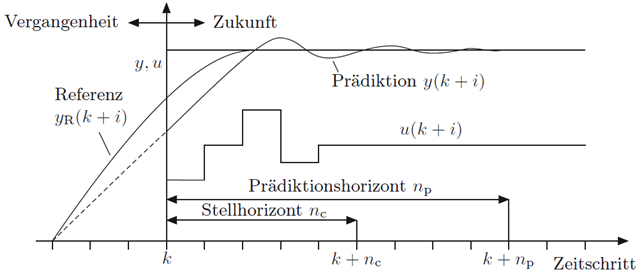
\includegraphics[width=0.7\textwidth]{figures/2_Grundlagen/MPC_Diagramm.png}
    \caption{Ablauf einer modellprädiktiven Regelung \cite{adamy2014}}
    \label{fig:MPC}
\end{figure}
Der Ablauf einer modellprädiktiven Regelung, wie in Abbildung \ref{fig:MPC} zu sehen, kann in drei Punkte unterteilt werden \cite{camacho2013model}:
\begin{enumerate}
    \item Mithilfe eines Modells wird der Ausgang eines Systems für $k+n_{p}$ Zeitschritte (Prädiktionshorizont) vorausgesagt. Die Prädiktion basiert sowohl auf den vergangenen Ein- und Ausgängen als auch auf den zukünftigen Eingaben über die Länge des Stellhorizonts $n_{c}$
    \item Die Stellgrößensequenz $u$ wird berechnet. Dabei wird eine Kostenfunktion minimiert, welche so gewählt wird, dass sich ein gewünschtes Systemverhalten einstellt. Der Stellaufwand wird in der Regel in der Kostenfunktion mit berücksichtigt. Ebenfalls können Beschränkungen, von z.B. den Eingangsgrößen, berücksichtigt werden. Für jeden Zeitschritt wird so das OCP gelöst.
    \item Das erste Element des Stellhorizonts wird auf das System angewendet. Stell- und Prädiktionshorizont verschieben sich um einen Zeitschritt in die Zukunft. Der Zyklus beginnt von vorn. 
\end{enumerate}
\subsection{Pfadfolgeregelung}
Die Implementierung der Pfadfolgeregelung für die in diesem Praktikum eine Teststrategie implementiert werden soll, ist in Abbildung \ref{fig:MPFC_Schema} dargestellt. Als Eingänge dienen der MPFC eine Sollgeschwindigkeit, Pfaddaten, Fahrzeugzustände, vorgegebene Beschränkungen und ein Fahrzeugmodell. Daraus werden eine Sollbeschleunigung und eine Solllenkradwinkelgeschwindigkeit berechnet.

Die Grundidee der Pfadfolgeregelung ist in \cite{Faulwasser2009} beschrieben: Der Regler soll einem vorgegebenem Pfad möglichst gut folgen. Die Geschwindigkeit entlang des Pfades wird, im Gegensatz zu trajektorienbasierten Ansätzen, bei denen die Geschwindigkeit an jedem Punkt des Pfades vorgegeben ist und eingeregelt werden soll, vom Regler selbst festgelegt. Durch die Implementierung wird ein konvergieren des Pfades auf den Sollpfad sichergestellt \cite{ritschel2019}.

Eine Methode zur Ermittlung geeigneter Parameter für das Optimierungsproblem der Pfadfolgeregelung ist in \cite{math11020465} dokumentiert. Darin steht die Erhöhung der Sicherheit und des Fahrkomfort im Fokus. Durch eine bayessche Optimierung werden Parameterwerte, welche eine gutes Verfolgen der Pfadgeschwindigkeit, geringe Abweichung vom Pfad und möglichst geringe laterale sowie longitudinale Beschleunigungen erzeugen, gefunden. Letzteres ist ein großer Faktor wenn es um Fahrkomfort geht \cite{BELLEM201890}.
\begin{figure}[H]
    \centering
    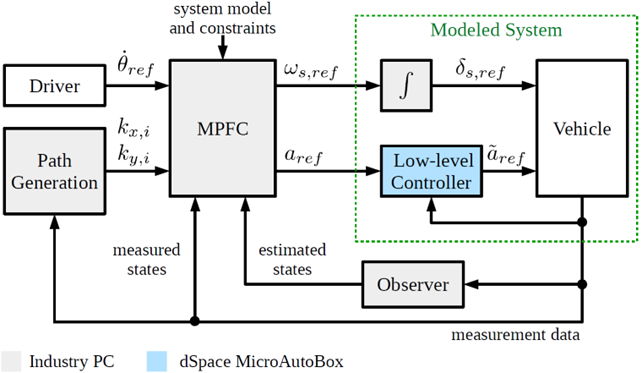
\includegraphics[width=0.7\textwidth]{figures/2_Grundlagen/MPFC_Schema.png}
    \caption{schematischer Aufbau der MPFC \cite{ritschel2019}}
    \label{fig:MPFC_Schema}
\end{figure}
    
\section{Szenariobasiertes Testen im Automobilbereich} \label{sec:SoftwaretestsAutomobil}

Um ein autonomes Fahrsystem zu realisieren und Sicherheit zu gewährleisten sind ausgiebige Test- und Verifikationsprozesse erforderlich. Dabei ist es nicht mehr ausreichend, Testdaten durch reale Testfahrten auf der Straße zu sammeln. Ein großer Anteil der Daten ist schlichtweg uninteressant, da keine kritischen Fahrsituation auftreten. Es bietet sich daher an, in einer Datenbank die kritischen Szenarien zu erfassen und für spätere Verifikationsprozesse wieder heranzuziehen \cite{Nalic2020}.

Um Szenarien zu beschreiben und in eine Datenbank einordnen zu können müssen diese klassifiziert werden. Eine Möglichkeit dafür ist die Einteilung nach Informationslevel \cite{Nalic2020}\cite{Bagschik2018}.
\begin{figure}[H]
    \centering
    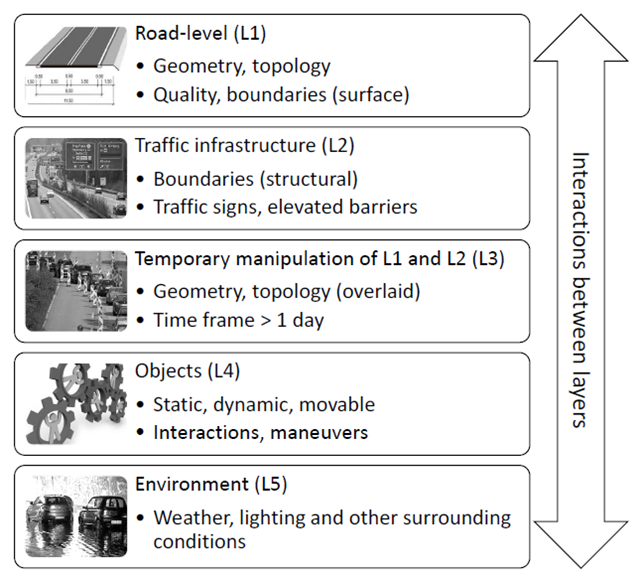
\includegraphics[width=0.5\textwidth]{figures/2_Grundlagen/layer_model.png}
    \caption{Einteilung des Informationsgehalts eines Szenarios nach Schichten \cite{Bagschik2018}}
    \label{fig:layer_model}
\end{figure}
Die erste Ebene definiert dabei grundlegende Eigenschaften der Straße, wie etwa deren Beschaffenheit oder Grenzen. Die nächste Ebene fügt Infrastrukturobjekte wie Straßenschilder hinzu. Ebene drei enthält Informationen über temporäre Veränderungen der darunterliegenden Ebenen. Ebene vier fügt einem Szenario statische und dynamische Objekte wie andere Verkehrsteilnehmer und Manöverplanung hinzu. Zum Schluss können noch Umweltfaktoren eingefügt werden \cite{Bagschik2018}.

Eine weitere Klassifizierungsmöglichkeit ist nach dem Detailgrad, wie es in Abbildung \ref{fig:scenario_level} \cite{Nalic2020}\cite{menzel2018scenarios}. Zunächst werden funktionale Szenarios beschrieben. Diese können einfach mit Worten beschrieben werden und enthalten noch keine Information über die Parameter. In einem ersten Abstrahierungsschritt werden diese zu logischen Szenarios. Hier wurden Parameter identifiziert und Grenzen für diese festgelegt. Um ein konkretes Szenario zu erhalten muss für jeden Parameter ein Wert ausgewählt werden. Theoretisch ermöglicht dies eine unendliche Anzahl an konkreten Szenarios, welche aus lediglich einem funktionalen Szenario erstellt werden können. Selbst bei rein simulativen Tests ist das nicht umsetzbar und muss reduziert werden \cite{menzel2018scenarios}.
\begin{figure}
    \centering
    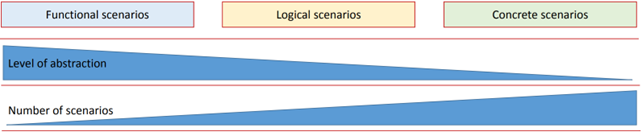
\includegraphics[width=0.7\textwidth]{figures/2_Grundlagen/scenario_level.png}
    \caption{Erhöhung der Anzahl an Szenarios mit zunehmener Konkretisierung der Szenarien \cite{menzel2018scenarios}}
    \label{fig:scenario_level}
\end{figure}

\section{Softwartests und CI/CD} \label{sec:CICD}

Ein geeignetes Testmanagement erhöht die Qualität einer Software maßgeblich. Ein Testprozess läuft in der Regel nach dem in Abbildung \ref{fig:testprozess} dargestellten Schema ab. Für den Testprozess exitisieren die Normen IEEE 829 und ISO-Standard 9126. Das International Software Testing Qualifications Board (ISTQB) arbeitet auf Grundlage dieser Normen an der Standardisierung von Systemtests \cite{witte2019testmanagement}.
\begin{figure}
    \centering
    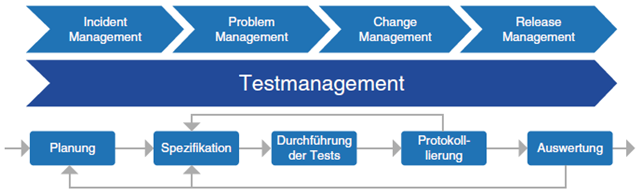
\includegraphics[width=0.7\textwidth]{figures/2_Grundlagen/testprozess.png}
    \caption{Ablauf eines Testprozesses \cite{witte2019testmanagement}}
    \label{fig:testprozess}
\end{figure}

Eine Möglichkeit Testprozesse Durchzuführen steckt hinter den Schlagworten Continuous Integration (CI) und Continuous Deployment (CD). Darunter versteht sich ein Prozess zum entwickeln, testen und freigeben von Software unter Nutzung von Versionsverwaltungssoftware wie er in Abbildung \ref{fig:ci-cd-flow-desktop} dargestellt ist. Wenn ein Entwickler in einem Softwaremodul Änderungen veranlasst, läuft ein automatischer Testprozess ab. Dieser ist typischerweise in Stages unterteilt, in Abbildung \ref{fig:ci-cd-flow-desktop} sind diese BUILD, TEST, MERGE. Werden darin keine Fehler in der Software gefunden werden die Änderungen eines Moduls zusammen mit den Änderungen an allen Modulen zusammengefasst und und somit die gesamte Software auf den aktuellen Stand gebracht (Continuous Delivery). Werden für die Gesamtsoftware ebenfalls keine Fehler gefunden kann eine neue Softwareversion zum Kunden gebracht werden (Continuous Deployment). Dieser Testprozess läuft in der Regel automatisch ab und veringert die Anzahl an Fehlern in Software \cite{redhat2024}.
\begin{figure}
    \centering
    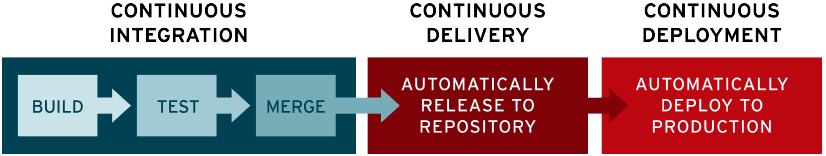
\includegraphics[width=0.7\textwidth]{figures/2_Grundlagen/ci-cd-flow-desktop.png}
    \caption{Ablauf eines CI/CD Prozesses \cite{redhat2024}}
    \label{fig:ci-cd-flow-desktop}
\end{figure}